\chapter{Wstęp}

\section{Cel projektu}
Celem projektu jest stworzenie aplikacji webowej do zleceń dla transportów okazjonalnych, która zoptymalizuje procesy logistyczne i wyeliminuje nieefektywne wykorzystanie zasobów transportowych. Aplikacja umożliwi użytkownikom łatwe i szybkie znalezienie odpowiedniego przewoźnika lub zleceniodawcy, co spowoduje redukcje pustych przebiegów i tym samym kosztów transportu.
Główne cele projektu:
\begin{enumerate}[labelwidth=\widthof{\ref{last-item}},label=\arabic*.]
\item Optymalizacja procesów logistycznych: Poprzez automatyzację procesu wyszukiwania i dopasowywania zleceń transportowych, aplikacja usprawni komunikację między zleceniodawcami a przewoźnikami, skracając czas potrzebny na znalezienie odpowiedniego transportu.
\item Eliminacja pustych przebiegów: Aplikacja umożliwi przewoźnikom znalezienie ładunków na trasach powrotnych, co zmniejszy liczbę pustych przebiegów i przyczyni się do oszczędności paliwa, co zredukuje koszty.
\item Redukcja kosztów transportu: Dzięki lepszemu dopasowaniu potencjalnych kontrahentów dla usług transportowych, aplikacja pozwoli na obniżenie kosztów transportu zarówno dla zleceniodawców, jak i przewoźników.
\item Poprawa bezpieczeństwa i jakości usług: Aplikacja umożliwi weryfikację kwalifikacji przewoźników oraz ocenę jakości świadczonych usług, co przyczyni się do zwiększenia bezpieczeństwa i zadowolenia klientów.
\item Ułatwienie dostępu do rynku transportowego: Aplikacja stworzy platformę, która ułatwi zarówno doświadczonym przewoźnikom, jak i nowym podmiotom na rynku. \label{last-item}
\end{enumerate}

Realizacja tych celów przyczyni się do stworzenia nowoczesnej i efektywnej aplikacji, która wspomoże rynek zleceń transportowych, przynosząc korzyści zarówno dla zleceniodawców, jak i przewoźników.

\section{Transport okazjonalny}
Transport okazjonalny to przewóz towarów, który nie spełnia definicji przewozu regularnego. Oznacza to, że odbywa się on bez ustalonego z góry rozkładu jazdy i może dotyczyć zarówno tras krajowych, jak i międzynarodowych.
Charakteryzuje się on:
\begin{itemize}
\item Brakiem stałego rozkładu jazdy. Pojazdy wykonują swoje trasy w zależności od zapotrzebowania klientów.
\item Jest inicjowany przez zleceniodawce. Przewóz zlecany jest na potrzebę klienta, nie określna on jednak, dokładnego terminu odbycia trasy.
\end{itemize}

\section{Wymagania niefunkcjonalne}
\begin{enumerate}[labelwidth=\widthof{\ref{last-item}},label=\arabic*.]
\item Innowacyjność: Wykorzystanie nowoczesnych technologii, takich jak \texttt{TypeScript}, \texttt{Next.js}, \texttt{Tailwind CSS}, \texttt{Node.js} oraz \texttt{PostgreSQL}, zapewni wysoką wydajność, skalowalność i bezpieczeństwo aplikacji.
\item Intuicyjny interfejs użytkownika: Aplikacja będzie posiadać prosty i intuicyjny interfejs użytkownika, który umożliwi łatwą obsługę zarówno dla zleceniodawców, jak i przewoźników.
\item Dostępność na różnych urządzeniach: Aplikacja będzie responsywna i dostosowana do różnych urządzeń, takich jak komputery, tablety i smartfony, co zapewni wygodę użytkowania w dowolnym miejscu i czasie.
\item Wielojęzyczność: Użytkownicy korzystający z aplikacji, będą mieli możliwość wyboru jednego z trzech przewidzianych języków: polski, angielski oraz niemiecki. Co przełoży się na międzynarodowy aspekt aplikacji.
\end{enumerate}

\section{Przypadki użycia}
\begin{figure}[ht]
	\centering
		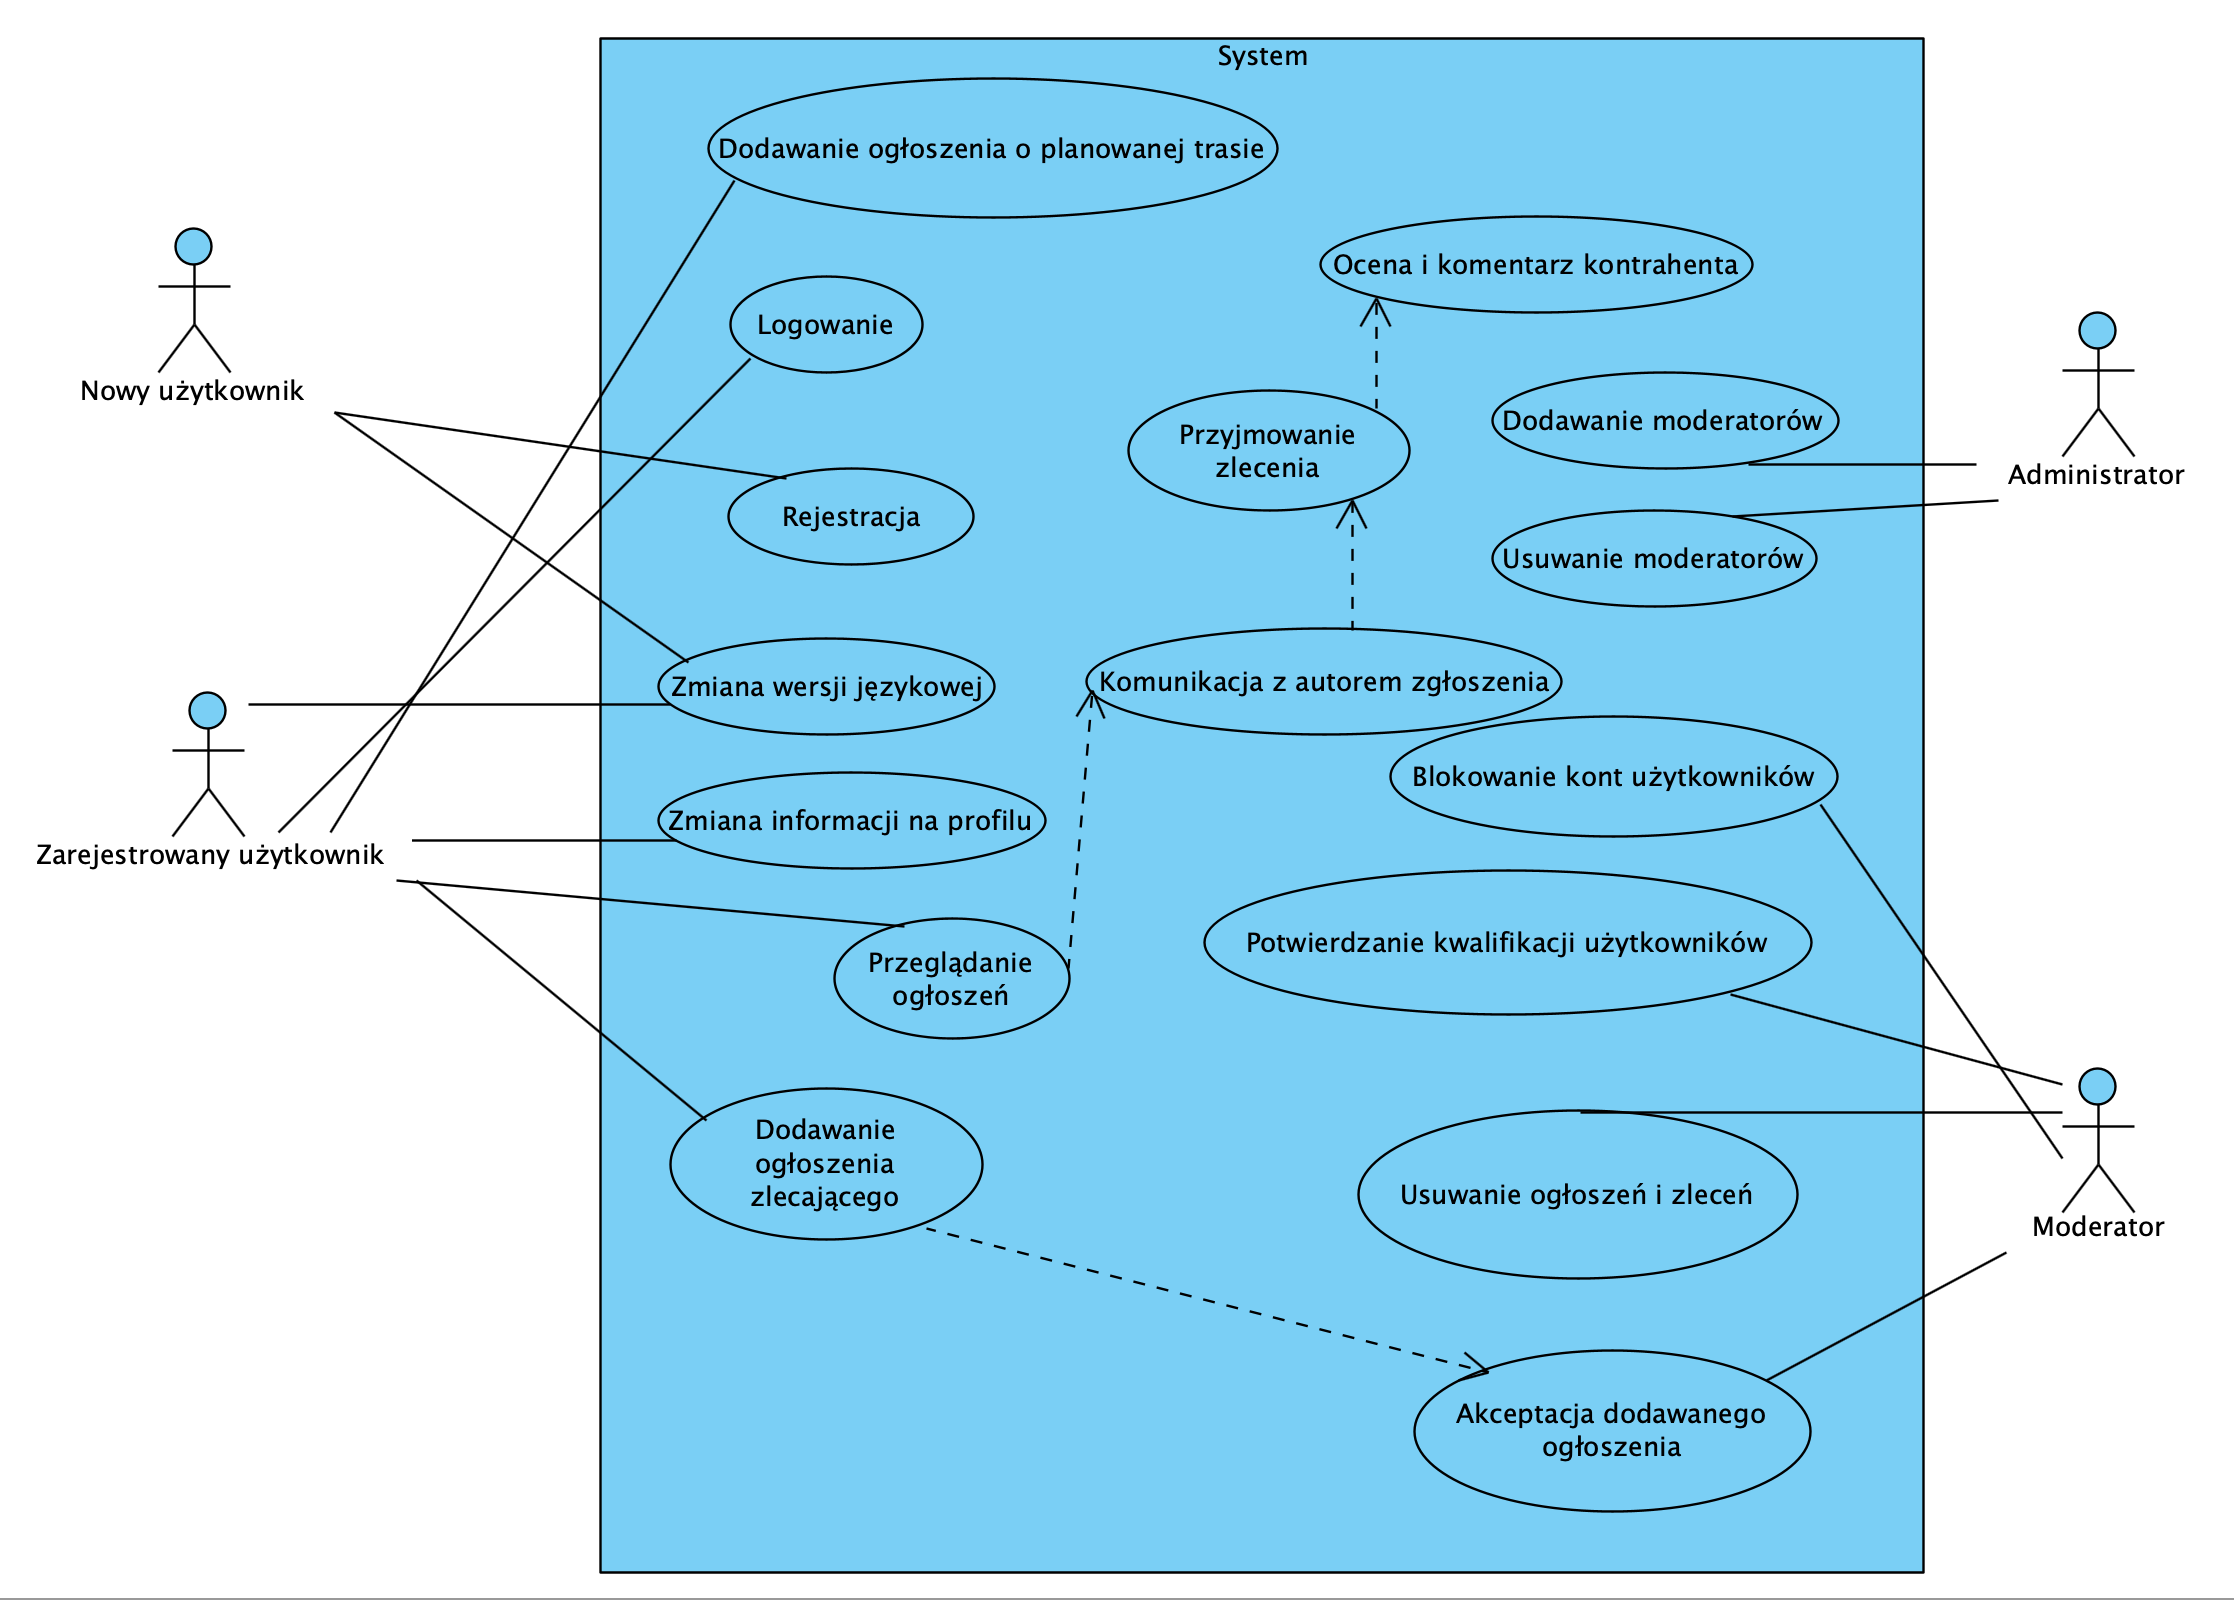
\includegraphics[width=0.9\linewidth]{rozdzial1/use_case.png}
	\caption{Przedstawienie przypadków użycia}
	\label{fig:Przedstawienie przypadków użycia}
\end{figure}
